%The interaction design of the clients, what principles has been used. Directed towards developers. Start with subsection here. Android and iOS need to start with subsubsection.

This chapter goes into detail on how the graphical and interactive parts of the clients are designed. It starts with a general view of the interaction design and then divideds into chapters based on the different clients.

\section{Desktop clients}
Screen clients use a tab based navigation between views, these tabs are shown at the top of the user interface. The common views in the current system are search, upload and process.

Search results are displayed in a table, experiments can be expanded to reveal the files contained in the experiment. The files in an experiment are grouped by types where each type consists of a row in the table that may be expanded to reveal the files of that type.

The upload view consists of experiment groups. Each experiment group contains a set of input fields for annotation and a list of files added to this experiment. The user may create new experiments in this view or add files to an existing experiment, multiple files may be added to multiple experiments simultaneously.

The base for the process view contains a set of input fields for the parameters that are to be used when processing a file.

\FloatBarrier
\subsection{Swing application}
The desktop application is constructed in a topdown approach that separates all the different functionalities into groups. Similar functions will be grouped together to utilize space.
The application is built with tabs that simplifies work by letting the user easily switch between different views. Each tab is described by appropriate name and contains related functionality.

The workspace tab lets the user easily manage files and experiments. It has easy access to the download and process functions.

The administration tab design is centered around to have different views that can be reached from the buttons on the left side of the screen. The the Annotations view is where you can add new annotations to the database. This view has a table of all current annotations in the middle of the screen and a toolbar on the right side. Additional functions can be reached from pop up windows when a user clicks on the buttons in the tool bar.
A principle in the design is when the user types in something wrong, an alert (popup) will be shown telling what went wrong and why, for example if the user did not type in a name of the annotation a popup telling that a annotation needs a name will be shown.  
\FloatBarrier



\FloatBarrier
\subsection{Web application}
Generally the design of the user interface for the web application is an integration of the principles previously described with core design elements of web and the twitter bootstrap element library.

The web client use a bootstrap styled navigation bar for main navigation where the navigation tabs look more like links in a web navigation bar. There are three types of views in the web client:

\begin{itemize}
	\item \textbf{Main views:} A main view covers the entire page. The structure among main views is shallow and the user may freely navigate between all main views using the navigation bar. Search and navigation are main views.
	\item \textbf{Sub views:} A main view may consist of several sub views. In this case the main view has a vertical navigation bar on the left side used to navigate between sub views, sub views may not be directly navigated outside of its main view. The user may navigate to other main views from a sub view. Except for the sub navigation bar the sub view covers the entire main view, replacing its content. There are sub views in the administration main view.
	\item \textbf{Modal views:} Modal views “rolls over” the current main view and are used for specialized operations. Modal views can navigated to using buttons inside main views and sub views. Usually the user will be taken back to the previous view when the modal is closed but navigation in a sequence of modal views could be implemented in the future. Processing of raw files is currently done in a modal view.
\end{itemize}

Content that belong together is grouped using so called "panels", a header that describes the content with an area for the content below, with everything wrapped up by a border.
The contrast between elements in the interface is of medium strength. Grayscale colors are used for most elements but elements that need to be highlighted or distinguished from other elements use colors. Colors with high saturation are used for highlighting and colors used for distinguishing elements have a lower saturation.

Buttons that perform actions always contain an icon and text so that the experienced user may more quickly perform the desired actions but finding buttons at a glance instead of reading button text.

\subsubsection{Search view}
The search view consists of two main parts, at the top there is a group of buttons for performing actions on files and experiments. This button group also contains the search query input and search button.

Below is a table where search results are shown. The table consists of different types of rows:

\begin{itemize}
	\item Experiment rows: These rows represent an experiment, they can be expanded to reveal the files contained in an experiment. The row has columns for the expand button, the experiment name and the annotations.
	\item File type rows: When an experiment is expanded three new rows are expanded, each representing one type of file. They can be expanded to reveal the files of that type that belong to the experiment. File column headers are also shown when a file row is expanded.
	\item File rows: These rows represent the files existing in an experiment. They have a checkbox that can be checked to select the file so that it can be used by the various actions exposed in the button group. File rows also have columns for file data.
\end{itemize}

\subsubsection{Upload view}
\begin{figure}[h]
\centering

\includegraphics[width=1\textwidth]{web_id_uploadFields.png}
\caption{\label{fig:web_id_uploadFields}Fields for experiment selection/creation.}
\end{figure}

The upload view has two states, first the user have to choose if it wants to create a new experiment to upload files or use an existing file. This step looks like \refer{fig:web_id_uploadFelds}.

\begin{figure}[h]
\centering
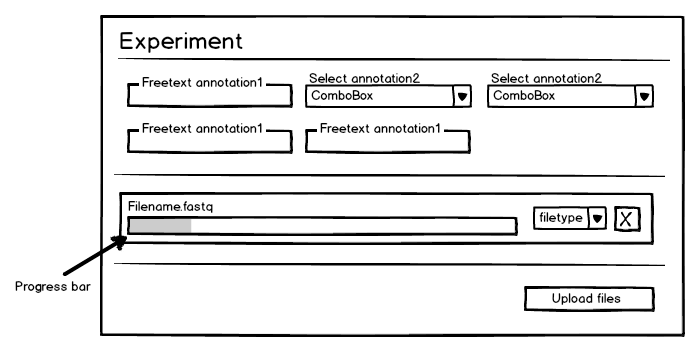
\includegraphics[width=1\textwidth]{web_id_fileUpload.png}
\caption{\label{fig:web_id_fileUpload}File upload and experiment annotation view.}
\end{figure}

Once the user has an experiment to upload files to it may start to upload files and annotate the experiment. The step for doing that looks like \refer{fig:web_id_fileUpload}.

\subsubsection{Process view}
The process view has a set of input and select fields for the user to input parameters to be used in the file processing. At the bottom of the view there’s a button used to start the processing.

\subsection{Systemadministration - Web}
The admin page is built up by four views: the navigation bar, the main view, the create annotation view and the edit annotation view. The first one is main view which consists of a navigation bar and a empty div-tag. 
The empty div-tag is then replaced with the annotation list view which has a Create new annotation button 
and a list of the available annotations on the database with an option to edit. 

When the user clicks on for example Create New Annotation, the div tag in the main view is replaced with the create annotation view.
The same goes for the Edit buttons on each annotation. This way we only have to render that specific div-tags current information 
and the navigation bar remains. 

The design is made so that the user should be able to avoid mistakes. For example in the 
create annotation page the user is not able to create an annotation without filling in all the fields. Futher more the 
field for Items in drop-down list is disabled if the user don't choose Drop-down list as the annotation type. 

In the Edit annotation view the same principles apply, but also there is a Delete Annotation button on this page which will
delete the entire annotation on the database. This made us ask two times if the user is sure of this action and ofcourse made the button red.

The back buttons on the different views work as any one using the internet is used to and the menubar option Annotations takes the user back to the main adminview.
\FloatBarrier
\section{Mobile clients}

\FloatBarrier
\subsection{Android}
The design of the android application is based on the design proposal suggested by the design team and our aim has been to recreate that look and feel. We did, however, find it necessary to take into consideration some of the android specific design paradigms which distinguish android applications from other smart phone platforms. For instance, the design put forth by the design group did not include a so called action bar   to the upper part of the user interface which are used for navigation. However, since these are fundamental to the structure of any android application, we were inclined to include this feature as a substitute for the slide-in menu described in the original design.

In the following sub-sections, we will compare the current design of our Android application (figures on the left) with the design proposal suggested by the design team (figures on the right), as well as attempt to explain our design desisions.


\subsection{Login View}
The two designs illustrated in figure \ref{fig:and_login} below are very similar except for the colour settings. There are textfields available for the user to type user name and password and a button to click when user is ready to log in. This is a popular layout for many login screens and thus a design many users are familiar with.


\begin{figure}[h]
\begin{center}


\begin{tabular}{c | c}
\addScaledImage{0.1}{andLogin.png} & \addScaledImage{0.47}{iosLogin.jpg} 
\end{tabular}
\caption{Android Login View vs iOS Design Proposal}
\end{center}
\label{fig:and_login}
\end{figure}


\subsection{Search View}
The two designs illustrated in figure \ref{fig:and_search} below are very similar. What is not depicted in the android view is the search button. It is, however, further down the item list and can be scrolled to.

\begin{figure}[h]
\begin{center}
\label{fig:and_search}

\begin{tabular}{c | c}
\addScaledImage{0.1}{andSearch.png} & \addScaledImage{0.47}{iosSearch.jpg} 
\end{tabular}
\caption{Android search view vs iOS design proposal}
\end{center}
\end{figure}


\subsection{Search Results View}
The two designs illustrated in figure \ref{fig:and_result} below are very similar except for the colour settings. The colour settings has changed since previous design since we adapted it to be more similar to the IOs design, which currently is designed using white background and black text. The list displaying search results is larger to facilitate usage for user and to take advantage of the screen space. It's easy to learn how to navigate the list. Scrolling is available if the list is long and if the user click on an experiment they are redirected to the experiment view displaying more information about that experiment.

\begin{figure}[h]
\label{fig:and_result}
\begin{center}
\begin{tabular}{c | c}
\addScaledImage{0.1}{andResult.png} & \addScaledImage{0.47}{iosResult.jpg} 
\end{tabular}
\caption{Android search result vs iOS design proposal}
\end{center}
\end{figure}

\subsection{Experiment View}
The two designs illustrated in figure \ref{fig:and_experiment} are similar except for colours and selection markers. The "slide bar" used for selection is not available in android and checkboxes has been used instead. All files for the experiment selected in the search result view is displayed here organised by data type. Checkboxes are commonly used and most users are familiar with how to handle them when making choices and selecting items. The button "Send to conversion" will be used to send selected files to the conversion view.

\begin{figure}[h]
\begin{center}
\label{fig:and_experiment}

\begin{tabular}{c | c}
\addScaledImage{0.1}{andExperiment.png} & \addScaledImage{0.47}{iosExperiment.jpg} 
\end{tabular}
\caption{Android experiment view vs iOS design proposal}
\end{center}
\end{figure}

\FloatBarrier
\subsection{iOS}

Focus has been on making a nice looking application with an intuitive workflow. The design is based on the design selected in the design phase. However, some changes has been made in order to follow the iOS design principles. New insights of the demands of the customer and our increasing experience has also resulted in improvements of the original design. Some of the design decisions are motivated in the text below.


\subsubsection{Navigation bar}
A navigation bar is used to make access to different main functionalities available at all times. The chosen design (at the end of the design phase) suggested to have an invisible menu which was slided in. However, an invisble menu is difficult to detect and does not follow the iOS design guidelines.


\subsubsection{Login Screen}
The login screen has two responsibilities; to make a nice first impression and to make it easy for the user to login. The design is kept simple and clean to avoid distractions.

\subsubsection{Search View}
The search view is designed to be usable for both advanced and new users. A list with available annotations is displayed to make it easy to do basic searches fast. Some annotations can only be selected with a picker view, while others are edited by typing free text. The reason for the occurance of the picker views is to simplify searches and help the user to make correct search requests. For example, the sex of an individual can only be male, female or unknown. Other values for the sex annotation would be nonsence!

\begin{figure}[ht]
\addScaledImage{0.2}{ios_search.png}
\caption{The search screen.}
\label{fig:ios_search2}
\end{figure}
\FloatBarrier

Each annotation has a corresponding switch button as seen in \refer{fig:ios_search2}. The button determines if the annotation should be included in the search request. This make it easy to make small changes to the search, while not clearing the annotation values.

The advanced user can customize the search query sent to the server. This gives the user the opportunity make more complex search queries and possibly make use of already accuried PubMed-search skills.

\subsubsection{Search Result View}
The main purpose of the search result view is to give an overview of the search results. The challenge with this view was to summarize large amount of information in a small area. The small screen of the iPhone made it impossible to have columns for each annotation. Instead a decision was made to group the files by experiment as seen in \refer{fig:ios_searchResult2}. The table with the experiments will only expand vertically, both when the number of shown annotations and the number of experiments grows. Thus, the user never has to scroll sideways which would be awkward.

\begin{figure}[ht]
\addScaledImage{0.2}{ios_searchResults.png}
\caption{The search result view.}
\label{fig:ios_searchResult2}
\end{figure}
\FloatBarrier

The user can choose which annotations to display in the result view. This gives the user the power to only show the annotations which are interesting at the moment. 

The file view (see \refer{fig:ios_files2}), which is shown when the user selects an experiment, only contains the most important information about the files of the specific experiment. The number of annotations shown in this view is kept at a minimun to avoid information overload and to give the user a good overview of the files. Three annotation were chosen: the name of the file, the date when the file was uploaded and the author. These were chosen to make it easy for the user to identify the correct files.

\begin{figure}[ht]
\addScaledImage{0.2}{ios_files.png}
\caption{The file view.}
\label{fig:ios_files2}
\end{figure}
\FloatBarrier

The functionality of the Convert files button can be reached from other views, but was added to this view as well to improve the workflow. Instead of first selecting the files, then going to the Selected files view and initiate the convertion from there, the user can now quickly convert files directly from the search results.


\paragraph{Selected Files}
The selected files view can be seen in \refer{fig:ios_selectedFiles2}. The files are grouped into four categories: raw, profile, region and other. This is done by showing each type of files in its own tab. The reason for this is to avoid the possibility to select files of different types since the tasks to perform are file type specific. It also gives a better overview of the files when only one type is shown instead of showing all files at the same time. Additionally, the top tab bar menu is following the iOS design guidelines.

\begin{figure}[ht]
\addScaledImage{0.2}{ios_selectedFiles.png}
\caption{The selected files view.}
\label{fig:ios_selectedFiles2}
\end{figure}
\FloatBarrier

\paragraph{Select task}
The select task menu can easily be expanded when new functionality is added to the application. The Execute-button is disabled as long as no task is selected. A checkmark is displayed next to the task to perform. When an other task is selected the checkmark is moved. The reason for not using switch buttons is that they would give the impression that several tasks could be executed at once, which is not possible at the moment.
